\newpage
\section{Voting on Proposals (On-Chain, Delegates)}
\label{sect:voting}

Once a properly signed proposal has been submitted on-chain, delegates may vote on whether or not to accept it.  A threshold is set for each vote.
As described in Section~\ref{sect:submission}, the thresholds for each proposal are included in the formal proposal at submission time.

\subsection{Voting}

Each \emph{registered} delegate (see Section~\ref{sect:registration}) may vote either in favour or against a proposal by submitting the corresponding transaction.  They may change their vote up to the point
where the vote is tallied.  Any changes after that point in time are not considered.  If a delegate chooses not to vote on a proposal, that is considered to be
a vote against the proposal.  Votes are submitted in the form of an on-chain transaction, and may incur fees.  The transaction needs to include:

\begin{center}
\begin{tabular}{||l|p{3in}|l||}
  \hline\hline
  proposal id & The unique identifier for the proposal, derived from the submission & 32 bytes
  \\\hline
  vote intention & Yes or no & 1 byte
  \\\hline
  Delegate public key hash & Unique identifier & 32 bytes
  \\\hline
  \hline
\end{tabular}
\end{center}

This ensures that there is a public and traceable record of each delegate's actual vote.


\subsection{Stake Snapshots}

Stake snapshots are taken at the start of each epoch.  These snapshots are currently used only for block production purposes, but they will be reused here for governance purposes.
The stake snapshot that is taken at the start of an epoch will be used for all delegated votes that are tallied at the end of the epoch.
The same stake snapshot that is used for block production is also used for endorsement.
As with block production, using fixed snapshots means that there will be a
slight delay before a change in stake will be effective for voting purposes.
However, this brings major efficiency advantages (it is not necessary to calculate specific snapshots per vote).

\begin{figure}
  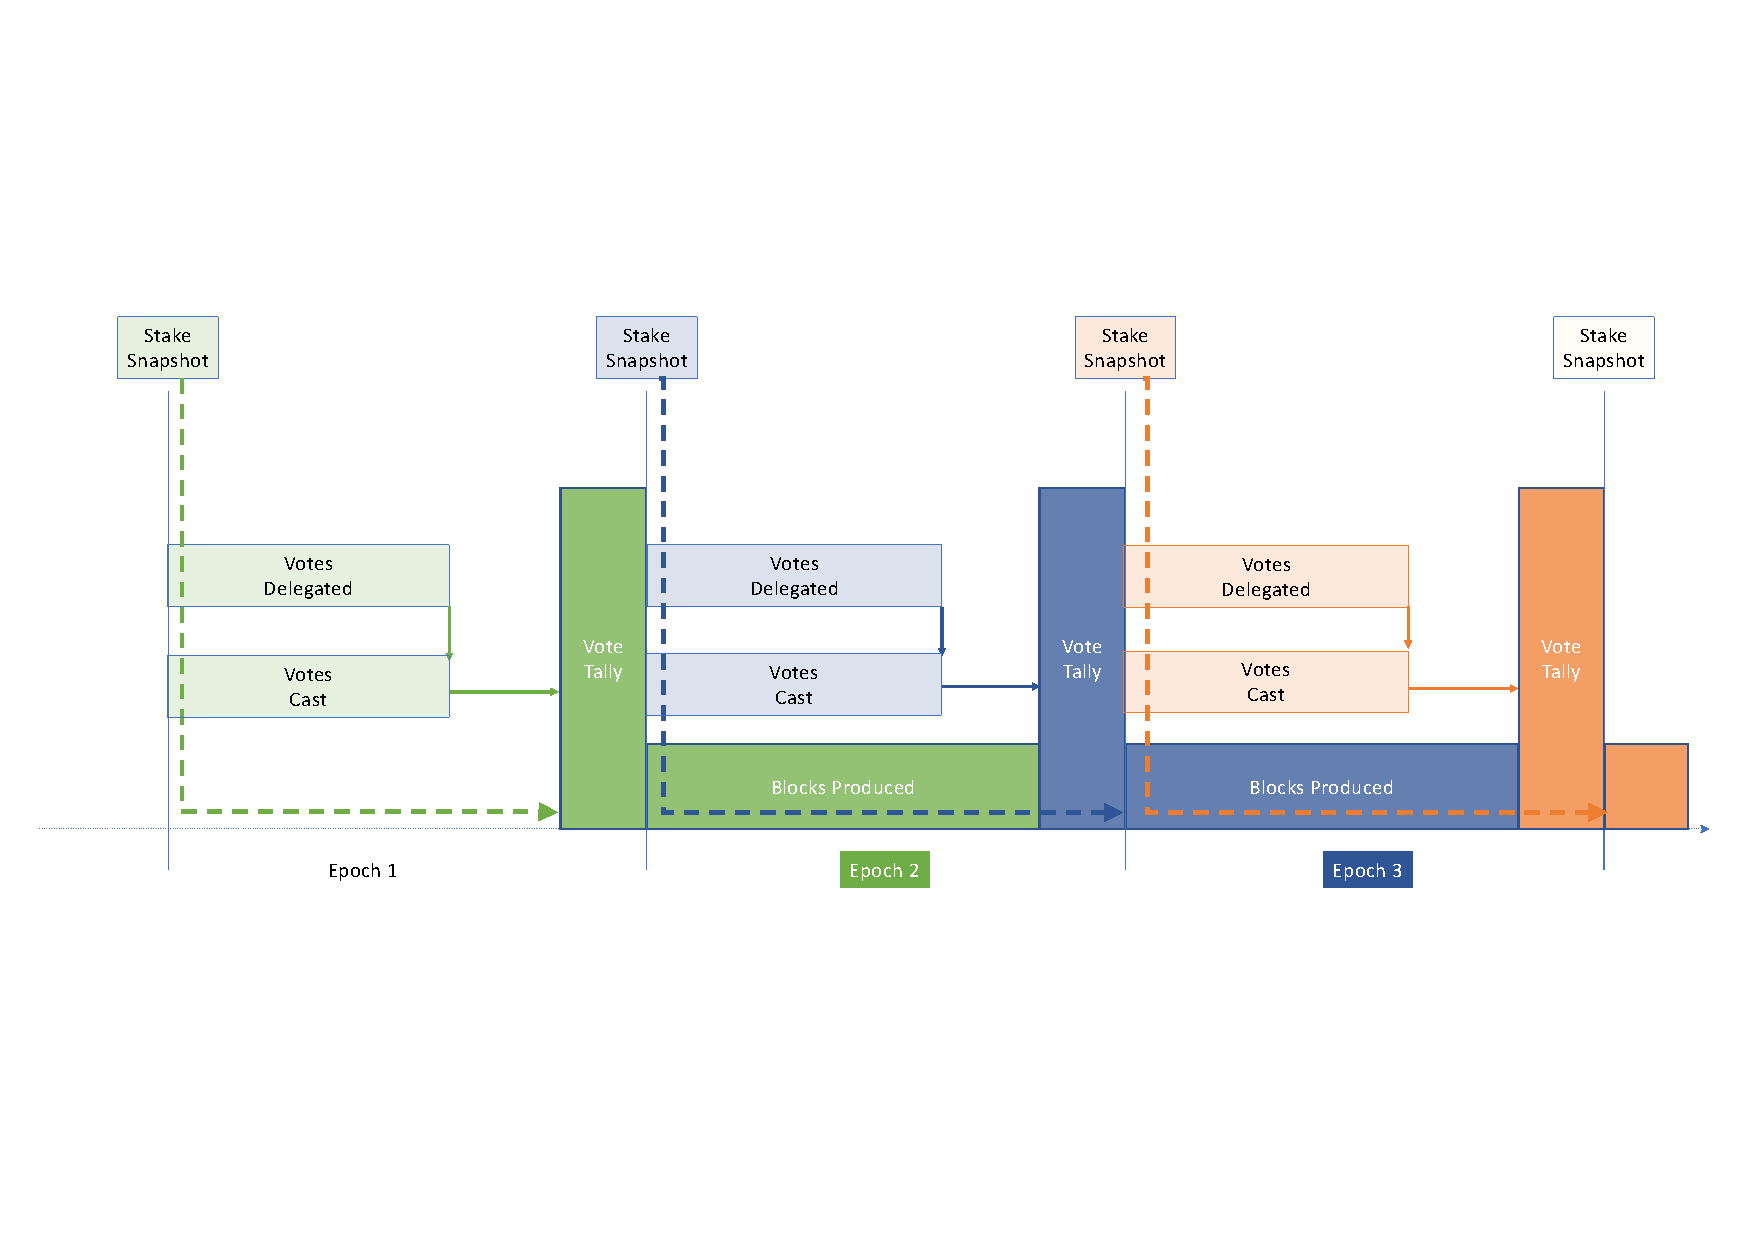
\includegraphics[trim=0 150 0 80,clip,width=\textwidth]{Stake-Snapshots}
  \caption{Stake Snapshots}
  \label{fig:stake-snapshots}
\end{figure}

\khcomment{It seems sensible to separate the vote and block production snapshots like this, but it does give a slightly odd effect, in that vote and block production stake
  will not always be the same in a given epoch.  They could be aligned, but then there will be a lag in the vote.}


\subsection{Tallying Votes}

Votes are tailied according to a snapshot of delegated vote that is taken at the specific point given in the proposal submission.  The stake snapshot from the start of the epoch is used to determine
the weight of each delegated vote for all votes that are tallied at the end of the epoch.  The total vote that is controlled by each delegate is the sum of all active delegations at the point that
the vote is tallied.  A calculation is made for the total amount of stake that is: i) explicitly in favour and; ii) explicitly against the proposal.  This is compared against the required voting thresholds and
if sufficient votes have been achieved, then the proposal will be accepted as decscibed below.\khcomment{Does the tally need to be recorded on chain?}

\subsection{Voting Outcomes and Thresholds}

Following the tally, a proposal may be either accepted or rejected, based on whether it has achieved the required voting threshold.  Any proposal that achieves at least
the specified percentage of votes is accepted, and passed forward for future enactment.
The threshold for accepting a specific vote is specified in the proposal\khcomment{there may also be minima that are set in the protocol parameters.}.
All thresholds are specified as a percentage of total ada.  There are a number of ways that this total can be specified.  In roughly declining order of size, these include:

\begin{enumerate}
\item
  The total ada that is in existence (i.e. 45 billion ada).
\item
  The total ada that is in circulation (i.e. that is not accounted in either the treasury or reserves pots).\khcomment{Preferred.}
\item
  The total ada that has been delegated for block production purposes in the current epoch.\khcomment{Preferred.}
\item
  The total ada that has been delegated for voting purposes in the current epoch.
\item
  The total ada that has been used to cast a vote on a specific proposal.
\end{enumerate}

A decision needs to be taken on how to determine the total that is used in a threshold calculation.\khcomment{It makes sense to use the same total for all votes rather than using different totals.}
Using the total ada in existence (option 1) means that very high voting thresholds cannot be achieved until all ada
is in circulation, and that ada that has not been circulated will always have a negative effect on voting.
This seems undesirable.
The second option avoids this issue, but means that ``inactive'' ada will count as a vote against a proposal, which may prevent the chain from making reasonable progress.
The third option ensures that all ``active'' participants in the blockchain are considered, but could in theory give results greater than 100\% (because of lag in the
block production snapshot compared with the voting snapshot, or if vote delegation is more popular than block production delegation).
While the fourth option may seem attractive, it may result in highly unrepresentative results if insufficient stake holders choose to delegate their vote.  This would potentially allow control of the
blockchain to be circumvented at low attack cost, so creating a security vulnerability, and would also create potential instability in the blockchain.
Likewise, the fifth option would allow proposals to pass with very little positive mandate (e.g. where only 10\% of the delegate group chose to vote on a specific issue, a majority vote could be
achieved with just over 5\% of the delegated stake).
The Priviledge project has developed further metrics that could be used to set the thresholds based on e.g. the proposal type and the
impact on the system.

\subsubsection*{Low Thresholds and Explicit Negative Voting}

One option is to require both positive and negative thresholds for a vote.  This might allow lower voting thresholds.
This approach has a number of disadvantages, however:

\begin{itemize}
\item
  The thresholds could not, anyway, be lowered significantly (or perhaps at all) without permitting unrepresentative outcomes in terms of
  favourable stake -- lower thresholds could only be accepted for certain kinds of proposal -- setting thresholds below 50\% would be hazardous, for example;
\item
  Delegates who control other delegation are already socially motivated to vote.  Delegators will remove their delegation from delegates who consistently fail to vote,
  and may require explanations for any proposal where no vote is given.
\item
  It imposes a per-vote transaction cost on normal ada holders who have chosen to register as their own delegates, and this may not be sustainable for small holders.
  This then works to reduce the number of ada holders who choose to register as delegates, consequently increasing centralisation\footnote{This assumes there is no compensation or incentive to encourage voting.}
  (Conversely, normal ada holders who do register as delegates must be positively in favour of/against a proposal by paying the requisite fee -- this acts as a deliberate drag
  to ensure some conservativism/stability in the system).
\item
  It adds complication and opportunities for gaming (eg with careful setting of thresholds);
\item
  Votes are registered on chain.  It may be socially unacceptable for a normal ada holder to vote explicitly against a proposal.  This allows an individual to have a ``silent'' negative vote.
\item
  Care needs to be taken over increasing execution costs. Tallies are potentially a critical point of performance failure, and this could perhaps double
  the cost for each tally.  High tally costs could even mean that some proposals were rejected (if they were not completed by the required deadlines, for example).
\end{itemize}
